\section{Feature Extraction Module}
The feature extraction module is to extract features to be able to distinguish one writer from the other.

We chose Local Binary Patterns as our feature extractor to extract features from the gray images of lines of each writer; LBP is a texture descriptor used to extract features by computing a local representation by comparing each pixel with its surrounding neighbors.

The first step in constructing the LBP texture descriptor is to convert the image to grayscale. We select a neighborhood of size r surrounding the center pixel for each pixel in the grayscale image. An LBP value is then calculated for this center pixel and stored in the output 2D array with the same width and height as the input image.

% figure 1
Figure \ref{fig:lbp_thresholding} The first step in constructing a LBP is to take the 8 pixel neighborhood surrounding a center pixel and threshold it to construct a set of 8 binary digits.

\begin{figure}
    \centering
    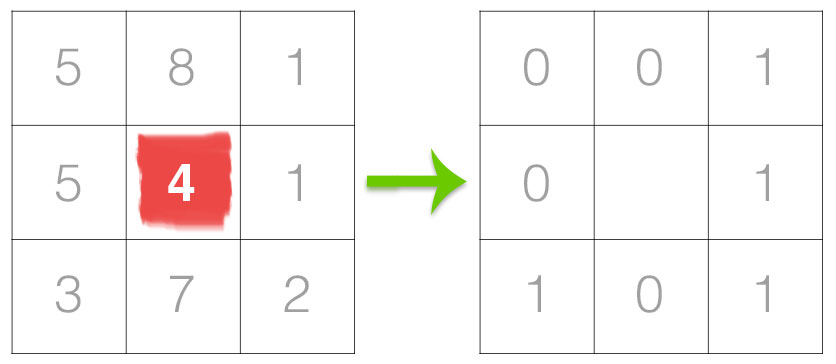
\includegraphics[width=0.9\linewidth]{lbp_thresholding}
    \caption{Constructing a set of 8 binary digits from the 8 neighbours surrounding the center.}
    \label{fig:lbp_thresholding}
\end{figure}

In this figure, the center colored by red, LBP checks if the intensity of the center pixel is greater-than-or-equal to its neighbor, then we set the value to 1; otherwise, we set it to 0

The second step is to calculate the LBP value for the center pixel by list the eight binary digits we got in the previous step and convert it to decimal, and we should list the binary digits by the same order and direction for every pixel in the dataset.

% figure 2
Figure \ref{fig:lbp_calculation} The Second step is taking the 8-bit binary neighborhood of the center pixel and converting it into a decimal.

\begin{figure}
    \centering
    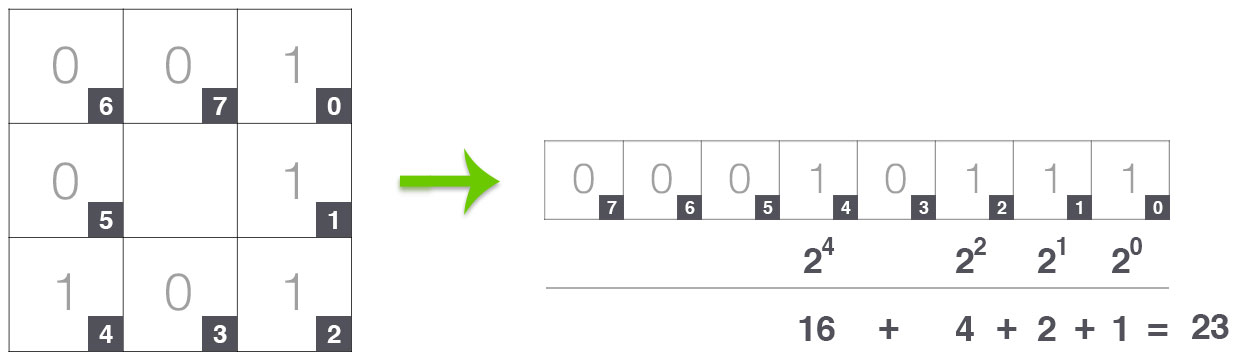
\includegraphics[width=0.9\linewidth]{lbp_calculation}
    \caption{Taking the 8-bit binary neighborhood of the center pixel and converting it into a decimal value.}
    \label{fig:lbp_calculation}
\end{figure}

% figure 3
Figure \ref{fig:lbp_to_output} Finally, yielding the LBP value and store it in the LBP output image.
\begin{figure}
    \centering
    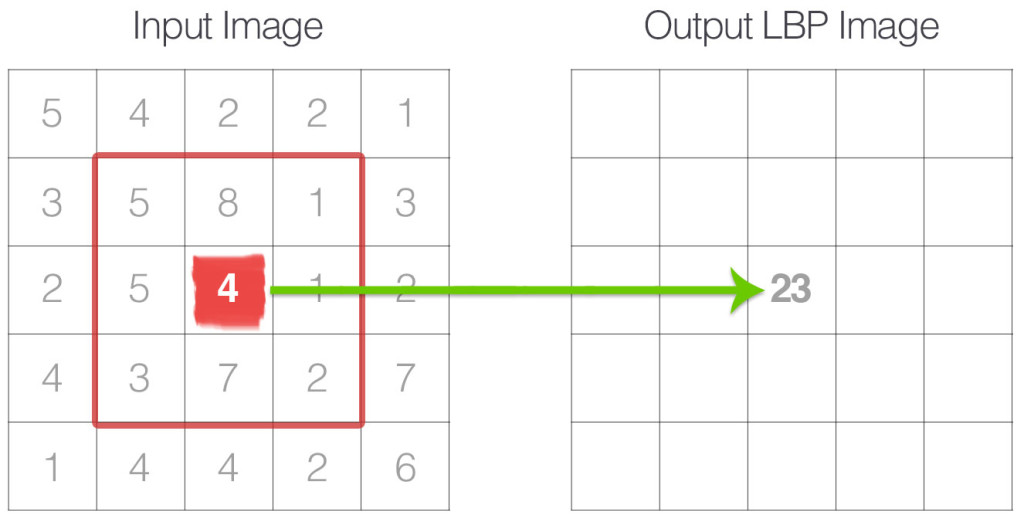
\includegraphics[width=0.9\linewidth]{lbp_to_output}
    \caption{The calculated LBP value is then stored in an output LBP image.}
    \label{fig:lbp_to_output}
\end{figure}

By fine-tuning the parameters of LBP such as the number of points \texttt{p} in a circularly symmetric neighborhood and the radius of the circle \texttt{r}
We chose radius equals 3 and 8 neighbors as it gives us the sweet spot between accuracy and speed. Another acceptable parameter will be four neighbors with a radius of 3. It also works very well with a little dropdown in the accuracy and less calculation time.
After calculating the LBP image, we get our feature vector by taking its histogram as our feature vector, and by trials, we found out that masking it with the binary image to calculate only the histogram for the black pixels in the binary image gives us better accuracy.
Moreover, because we have eight neighbors, we got $2 ^ 8 = 256$ possible patterns, so our LBP image has a minimum value of 0 and a maximum value of 255, allowing us to construct a 256-bin histogram of LBP codes as our final feature vector.
Finally, we normalize our feature vector by dividing it by its means.